% Chapter Template

\chapter{Evaluation}\label{ch:evaluation}


\section{Language Formalism Evaluation}\label{sec:language-formalism-evaluation}
% range of qs you can ask
% what class of contracts cannot be represented (which can well?)

% "what are the fundamental operators i need to represent a borad range of contrcts"


% come up with the bare-bones programming lang for contract rep

% Confis is not a parsimonious lang? or is it?

% "is it the min set of stuff we need?" clearly not -> but is what i have enough to represent a useful class of contracts


% I have demonstrated I can succesfully translate a class of contracts (by translating a couple)
% ^ mention in abstract

% normally you need to translate from a formalism into the other (symboleo to event calc fluents) then run model checkers etc
% whereas confis is self contained, no extra knowledge necessary

%

The Confis language formalism and semantics are discussed in~\autoref{sec:language-semantics}.
This project will evaluate it in how it meets the requirements described in~\autoref{sec:objectives}, its expressiveness (how capable it is to represent complex contracts) as well as how it performs in relation to comparable formalisms (like~\nameref{subsubsec:symboleo}~\cite{symboleo2020} or~\nameref{subsec:accord}~\cite{accordHomepage}).
Due to the nature of legal agreements (and the impossibility of formalising large amounts of existing legal contracts) this assessment is a qualitative one.

As for as fulfilling the accessibility requirements, Confis is one of the few formalisms in the literature that makes an effort to penetrate industry by
\begin{itemize}
    \item Making few assumptions about the user's background (including knowledge such as event fluidity, event calculus, or first order predicate logic).
    \item Choosing language constructs to purposefully resemble natural language.
    \item Providing additional tools to ease development and shorten the iteration loop.
\end{itemize}

The Query UI~(\autoref{sec:queryUI}), Confis-to-English conversion~(\autoref{sec:additional-tooling:doc-rendering}), the Confis Editor~(\autoref{sec:confis-editor}) and the structure of the Confis language itself (\autoref{sec:language-semantics}) were all developed with this goal in mind.

Exceptions to this statement include accessible technologies like Juro (\autoref{subsec:juro}).
Such tools add contract metadata without actually allowing for querying beyond fetching the metadata, nor attempt to capture the semantics of the agreement -- like Adobe Signing tools or typical Ricardian Contracts~\cite{ricardianWeb}, but unlike Symboleo or The Accord Project.

We translate to Confis a sample contract used in Symbolio~\cite{symboleo2020} in order to compare the same agreement in two different languages.
For the sake of brevity, we wille examine an extract~(given in~\autoref{tab:meat-confidentiality}), but the full original (in plain English) can be found at~\autoref{tab:meat}, the full Symbolio specification at~\autoref{fig:symbolio:meatSales}, and the full Confis agreement at~\autoref{fig:confis:meat}.
The translated extracts are both re-written self-contained examples (rather than text extracts from the original, longer contracts).
This is in order to fully reflect the necessary boilerplate and ceremony of each language.

\begin{table}[h]
    \centering
    \setlength{\fboxsep}{10pt}
    \fbox{
        \begin{minipage}{0.8\textwidth}
            \textbf{Confidentiality}
            \begin{enumerate}
                \item Both Seller and Buyer must keep the contents of this contract confidential during the execution of the contract and six months after the termination of the contract.
            \end{enumerate}
        \end{minipage}
    }
    \caption[Sample confidentiality clause]{Sample confidentiality clause, extracted from~\autoref{tab:meat}}
    \label{tab:meat-confidentiality}
\end{table}

\begin{listing}[h]
    \centering
    \begin{minted}[
        autogobble,
        frame=lines,
        framesep=2mm,
        fontsize=\footnotesize
    ]{kotlin}
val effDate = 1 of June year 2022
val reveal by action(
    description = "as in not keeping the contents confidential"
)
val contract by thing("the Contract", description = "this Agreement")
val seller by party("the Seller", description = "Alice Liddell")
val buyer by party("the Buyer", description = "The Meat Supermarket, Inc")

seller mayNot reveal(contract) asLongAs {
    within { effDate..(effDate + 6.months) }
}

buyer mayNot reveal(contract) asLongAs {
    within { effDate..(effDate + 6.months) }
}
    \end{minted}
    \caption{Confis for~\nameref{tab:meat-confidentiality}, extracted from~\autoref{fig:confis:meat}}
    \label{fig:confis:meat-confidentiality}
\end{listing}

\begin{listing}[h]
    \begin{minted}[
        autogobble,
        frame=lines,
        framesep=2mm,
        fontsize=\footnotesize
    ]{prolog}
        Domain meatSaleDomain
        Seller isA Role with returnAddress: String, name: String;
        Buyer isA Role with warehouse: String;
        Disclosed isAn Event;

        endDomain

        Contract MeatSale (buyer: Buyer, seller: Seller, effDate: Date)

        Declarations
        disclosed: Disclosed;

        Surviving Obligations
        so1 : Obligation(seller, buyer, true,
            not WhappensBefore(disclosed, Date.add(Activated(self), 6, months))
        );

        so2 : Obligation(buyer, seller, true,
            not WhappensBefore(disclosed, Date.add(Activated(self), 6, months))
        );
        endContract
    \end{minted}
    \caption{Symboleo Specification for~\nameref{tab:meat-confidentiality}, extracted from~\autoref{fig:symbolio:meatSales}}
    \label{fig:symbolio:meatSales-confidentiality}
\end{listing}

\paragraph{Specifying a legal Obligation}
Notice how Symboleo allows representing a more complex domain by specifying an \emph{Event} \texttt{`Disclosed'}, and constraining the legal capabilities of Buyer by creating an \emph{Obligation} (with a notion of this obligation being \emph{from} Buyer \emph{towards} Seller) which specifies that the \texttt{disclosed} event cannot happen before six months after the end of the contract.
In Symbolio's model if \texttt{disclosed} happen, the breach cannot be attributed to either Seller nor Buyer.

Confis specifies a simpler domain -- while it also specifies Seller and Buyer and represents `disclosing' as an Action, it has no notion of \emph{creditor} and \emph{lender} when it comes to Requirements (defined in~\autoref{def:requirement}).
On the other hand, Confis can `blame' specific parties for a breach, as it attributes Actions to Subjects.
Confis is also unable to keep track of its own execution time -- instead it requires specifying the date in the contract.
Notice how this abstracts away the document from the real-world execution date, and how this limitation of Symboleo is omitted in the original paper~\cite{symboleo2020}, but present in the sample source code~\cite{symboleoMeat}.

Both models are capable of expressing periods of time, but in Confis they are not part of the algebra (they are instead more general~\nameref{def:circumstance}s).

\paragraph{Accessibility}

While both contracts require language knowledge to write them, Confis can be read without prior training and its functions (\texttt{within}, \texttt{mayNot}, \texttt{asLongAs},~\dots) are easy to memorise.
The best example of this is the operation of summing six months to a time period -- while Symboleo requires specifying a \texttt{Date} library and wrapping the duration with a function (\texttt{`Date.add(..., 6, months)'}), Confis uses operator overloading to sum to a date (\texttt{`... + 6.months'}).

As far as readability goes, Confis goes the extra mile by trying to combine metadata and language semantics to provide an English-like preview.
This prose rendering is shown in~\autoref{fig:confis-render-meat-confidentiality}.
While the preview is not as clear as the original plain-English clause, it conveys the obligations of each party well and is unambiguous thanks to its definition referencing (which is common in real legal agreements).

\begin{figure}[H]
    \centering
    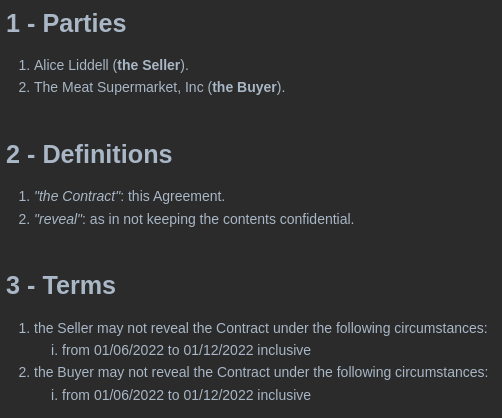
\includegraphics[width=0.67\columnwidth]{figures/confis.meat.prose}
    \caption{Confis prose rendering of~\autoref{tab:meat-confidentiality}}
    \label{fig:confis-render-meat-confidentiality}
\end{figure}

For a more detailed comparison of the specifications of this agreement in the Confis and Symboleo languages, please refer tor\autoref{ch:confis-examples}, in partcular~\autoref{subsec:meat-contract-comparison}.

\subsection{Confis Limitations in its Semantics}\label{subsec:confis-lang-limits}

While the focus Confis makes in Accessibility makes it easier to learn, read, and write;
it comes at a price in the guarantees it brings and the expressiveness of the contracts that it can represent.
% TODO solutions in future work?
This section provides a couple examples of clauses in existing contracts that Confis struggles to formalise and tries to generalise the situations it cannot encode, as well as suggesting solutions for the problem.

\subsubsection{Act Upon Violation}
\label{subsubsec:limits-violations}

Contracts are sometimes defensively written (not unlike defensive programming software engineering practices) where they may include clauses that specify what should happen upon breach of other clauses (an example of such a clause is given in~\autoref{tab:meat-breach}).

\begin{table}[h]
    \centering
    \setlength{\fboxsep}{10pt}
    \fbox{
        \begin{minipage}{0.9\textwidth}
            \textbf{Payment \& Delivery}
            \begin{itemize}
                \item In the event of late payment of the amount owed due, the Buyer shall pay interests equal to <intRate> the Seller may suspend performance of all of its obligations under the agreement until payment of amounts due has been received in full.
            \end{itemize}
        \end{minipage}
    }
    \caption[Sample breach clause]{Sample breach clause, extracted from~\autoref{tab:meat}}
    \label{tab:meat-breach}
\end{table}

In Confis semantics, this represents a contradiction in the logic of the contract, because we have a rule specifying that a set of states is a breach, and then other rules specifying capabilities when in those states.
This compromise between contradiction detection (extremely useful for helping the drafter produce well-formed contracts) and expressiveness (allowing these do-in-case-of-breach clauses) is unavoidable in the current semantics of Confis Allowance~(see~\nameref{def:allowance} for more details).

In order to circumvent this limitation, it is possible to create two `cases': a Permission that allows paying on time, and different Permission that allows paying at any time with interest.
While this removes the contradiction, it does not capture the violation semantics of the original legal agreement.

Symboleo is capable of capturing such a scenario thanks to its \texttt{Happens(Violated(\_))} predicate, which can create a new obligation when a different obligation is violated.

\subsubsection{Confis Does Not Have Time in its Event Algebra}
\label{subsubsec:limits-time}

Symboleo (and other logic-based solutions like~\cite{knottenbeltContractDriven}) relate events through \emph{happensBefore} partial orderings (introduced by~\cite{kowalski1989logicEventBased}).
They then can use these relations to model enforcing conditions, pre-conditions, and post-conditions over periods of time.

Confis only has a concept of time as a~\nameref{def:circumstance} -- an event does not necessarily happen at a given time, the same way it does not necessarily happen with a given purpose.
Ordering of events is established with an additional circumstance called a Past Action.
Again, this Circumstance does not receive special treatment and like the others it is up to the author of the contract to specify it.

While this design choice greatly simplifies rule generation and language semantics (thus making Confis easier to learn) it is a sacrifice in expressiveness.

For example, unlike Symboleo, Confis is unable to allow a new Capability only after an event $E$ occurred at a time $t$ and $E$ has happened after another event $E_{\text{past}}$.
Instead, Confis only allows a new capability after $E$ and $E_{\text{past}}$ have both happened, regardless of whether $E$ happened at time $t$, or whether $E$ happened before or after $E_{\text{past}}$.

It is possible to mitigate this issue by explicitly forbidding $E_{\text{past}}$ to happen before $E$ -- but then we would be slightly altering the original contract's semantics by introducing a new clause breach scenario.

\subsubsection{Confis Does Not Model Amounts}
\label{subsubsec:limits-amounts}

A key barrier to accessibility in existing formalisms -- and even any general-purpose programming language -- is their type systems.
Other than the absolutely necessary abstractions for the domain (such as Parties or Actions) users need to know what a strictly positive integer or a floating point number are.
The language then usually needs to define operations on these types, as well as extend them with other types such as Dates, Lists, etc.

Confis lowers the entry barrier by doing without most of this mental overhead (the only type concerned with numerical values it allows is a Date).
It does not require using libraries in order to perform operations -- mostly because there are no such operations, but partly thanks to operator overloading like in \autoref{fig:confis:meat-confidentiality}.

This greatly limits its expressiveness in terms of numerical amounts and the computations that can be done on them during the contract evaluation.
Consider The Accord Project~\cite{accordHomepage}~(see~\autoref{subsec:accord}), which models programs computationally with a more general-purpose language.
It is able to perform complex floating-point arithmetic in order to compute interest rates and fees, such as the one given in~\autoref{tab:economist-interest}.

On the other hand, Symboleo (and similar logic-based technologies) struggle more to perform such time-based calculations (possibly due to their declarative nature).
In the original Symboleo paper~\cite{symboleo2020} which contains a meat sales example hand-picked to showcase the language, the authors do not attempt to perform an interest calculation over time even though their original agreement (given in~\autoref{tab:meat}) specifies one -- this is shown in~\autoref{fig:symbolio:meat-interest} for convenience.

\begin{listing}[h]
    \centering
    \begin{minipage}{0.85\textwidth}
        \begin{minted}[
            autogobble,
            frame=lines,
            framesep=2mm,
            fontsize=\small
        ]{prolog}
        Domain
        Currency isAn Enumeration(CAD, USD, EUR);
        PaidLate isAn Event with
            amount: Number, currency: Currency, from: Buyer, to: Seller;

        Contract MeatSale (
            buyer : Buyer,
            seller : Seller,
            curr : Currency,
            interestRate: Number
        )

        endDomain

        Declarations
        paidLate: PaidLate with
            % where interestRate is a constant
            amount := (1 + interestRate / Math.abs(2)),
            currency := curr,
            from := buyer,
            to := seller;
        \end{minted}
    \end{minipage}
    \caption{Symboleo extract from~\autoref{fig:symbolio:meatSales} concerned with interest rates}
    \label{fig:symbolio:meat-interest}
\end{listing}

In short, while Confis lacks the computational capabilities of a programming language, it is not lacking when compared to Symboleo since it does allow specifying numerical constants (except without having to specify their types).
Additionally, traditional contracts also tend to leave to the reader such computations.

\begin{table}[h]
    \centering
    \setlength{\fboxsep}{10pt}
    \fbox{
        \begin{minipage}{0.9\textwidth}
            \textbf{Payment Terms}
            \begin{itemize}
                \item
                \ [\dots]
                Payments made after the due date may be [\dots] subject to a late fee equal to the lesser of 1.5\% per month or the maximum allowed by law.
            \end{itemize}
        \end{minipage}
    }
    \caption[The Econoimist licence interest rate clause]{Clause concerning an interest rate, extracted from~\cite{economistIU2016licence}, a Licence Agreement by The Economist Group}
    \label{tab:economist-interest}
\end{table}

\subsubsection{Confis Circumstances Are Domain-Aware}
\label{subsubsec:limits-domain-circumstances}

A Circumstance is an instance of an object that implements the functions given in~\autoref{def:circumstance}.
These operations vary greatly depending on the domain that the Circumstance is meant to represent.
For example, for time-type Circumstances, the \texttt{overlapsWith} function checks for overlaps in time ranges;
while in past-event-type Circumstances \texttt{overlapsWith} checks the union of the sets of past events.
This makes Circumstances very intuitive to use in practice: if the contract specifies Alice must pay this week and she paid this Monday, she expects `Monday' to be generalised by `this week', without needing to learn about the abstractions behind Circumstances.


The price to be paid for this ease-of-use is that Circumstances for new domains must be implemented before they can be used.
The most simple example is geographical locations.
This Circumstance is not already built into Confis.
If we were to make such an extension to the language, we would need to define a location-type circumstance as some coordinates (or perhaps an address).
The functions \texttt{generalises} and \texttt{overlapsWith} would compare coordinates in order to determine if one is a location included in the other (say, a house within a street), or if they are close enough to be the same place.

In short, making domains accessible at the language level requires less general abstractions that require domain knowledge at the implementation level.
While Confis is built to be easily extensible implementation-wise, this is a rare limitation in specification languages, which usually aim to be as general as possible in order to cover all possible cases.
The trade-off is once again in accessibility and expressiveness, and can be circumvented by encoding a Circumstance inside a~\nameref{def:sentence}'s~\nameref{def:action} -- following the previous example, rather than `deliver', the Action can be rewritten as `deliver to 10 Downing St.'.

\subsection{Gravity of Language Semantics Limitations}\label{subsec:gravity--lang-limits}

This subsection aims to determine to what extent the limitations presented in~\autoref{subsec:confis-lang-limits} affect negatively the practical usability of Confis.
Given how Confis is superior in its accessibility to comparable languages in the literature like Symboleo and The Accord Project (by virtue of the compromises it makes) we have focused on comparing real-world contracts with their Confis representations, including~\cite{economistIU2016licence, symboleoMeat, jetbrainsToolbox, seismicDataLicence}.

The main discrepancies between the intended meaning of the plaintext agreements and their Confis counterparts concern re-evaluation of legal capabilities and obligations (ie, Confis'~\nameref{def:permission} and~\nameref{def:requirement}) when the state-of-the-world changes.
This includes the~\nameref{subsubsec:limits-violations} and~\nameref{subsubsec:limits-time} limitations.
Other lacks in expressiveness (like~\nameref{subsubsec:limits-domain-circumstances}) can be more easily circumvented by adapting Sentences to convey the intended meaning and by splitting clauses into several such Sentences.

Full examples of such discrepancies can be found in the code archive, as well as in~\autoref{ch:confis-examples}.
We come to the conclusion that, despite the shortcomings of Confis as previously listed, we successfully represented the aforementioned contracts in the Confis specification.

\section{Software Deliverables}\label{sec:software-deliverables}

Key software components like the language implementation, rule generation, and legal prose rendering have been thoroughly tested for correctness through unit and integration tests, in the spirit of rigorous software engineering.
The methodology used in integration tests involves drafting plaintext contracts with the DSL implementation and comparing the contract and the internal representation it produces, as well as comparing the internal representation and the responses to different queries (which stem from rules generated from said internal representation).
A brief test coverage report can be found in~\autoref{tab:coverage}

\begin{table}[h]
    \centering
    \setlength{\tabcolsep}{8pt} % Default value: 6pt
    \renewcommand{\arraystretch}{1.2} % Default value: 1
    \begin{tabular}{l|c}
        \hline
        \textbf{Component}            & \textbf{Coverage} \\
        \hline
        \hline
        Language implementation       & 90.6\%            \\
        \hline
        Rule generation \& Evaluation & 85.0\%            \\
        \hline
        Natural language rendering    & 94.2\%            \\
        \hline
        Internal representation       & 73.5\%            \\
        \hline
    \end{tabular}
    \caption{Coverage for Confis components}
    \label{tab:coverage}
\end{table}

%Comparing implementations of contract specification languages is outside the scope of this project.
Some deliverables of other specification languages (like the querying engine) are left unimplemented by competing technologies like Symboleo~\cite{symboleo2020}, therefore it is hard to perform quantitative comparisons.

In order to still demonstrate the tractability and the practical applicability of the computations Confis performs, we measure compilation time and evaluation time of a Confis agreement.
We measure the following:
\begin{itemize}
    \item \textbf{Kotlin compilation time}, which converts text to a compiled Kotlin binary.
    \item \textbf{IR generation}, which converts Kotlin binaries to the Confis IR
    \item \textbf{Rule generation and evaluation}, which converts Confis IR to Easy Rules, and then evaluates the rules according to a given query (for all three kinds of queries)
\end{itemize}

The specifications of the machine these measurements are performed on are given in~\autoref{tab:measurement-env}.

\begin{table}[h]
    \centering
    \begin{tabular}{l l}
        \hline
        \textbf{Hardware Model}  & Dell XPS 9300                  \\
        \textbf{Processor}       & 1 core of Intel Core i7-1065G7 \\
        \textbf{OS}              & Linux 5.18.3                   \\
        \textbf{JVM}             & OpenJDK RE (build 11.0.15+10)  \\
        \textbf{Kotlin Compiler} & version 1.7.0                  \\
        \hline

    \end{tabular}
    \caption{Specifications of host environment for performance evaluation}
    \label{tab:measurement-env}
\end{table}

The methodology is as follows:
\begin{itemize}
    \item We evaluate the Confis agreements \texttt{minimal}~(see~\autoref{fig:confis:minimal}), \texttt{geophys}~(see~\autoref{fig:confis:geophys}), and~\texttt{meat}~(see~\autoref{fig:confis:meat}).
    \item No compilation caching of any kind is used (although the prototype does support caching)
    \item We measure Kotlin compilation, IR generation, and rule generation and evaluation (for all three query types discussed in~\autoref{sec:rule-generation}).
    We evaluate rule generation and evaluation as a single measurement because they are both query-dependent (different rules are generated for different queries).
    \item To average out random variations caused by the kernel scheduler, we perform the measurements 100 and report the averages.
    \item Measurements are performed on a warm JVM~\cite{venners1998java}.
    \item Confis code will be loaded into memory before measuring, so that fetching from disk is not taken into account.
\end{itemize}

The results of these measurements can be found in~\autoref{tab:benchmark-results}.
Please refer to the code archive for the benchmarking code\footnote{
    The code that performs the benchmarks can be found under:
    \begin{itemize}
        \item \texttt{script/src/test/kotlin/scripting/PerformanceTests.kt}
    \end{itemize}
}.

\begin{table}[h]
    \centering
    \begin{tabular}{|l|c|c|c|}
        \hline
        \multicolumn{1}{|c|}{\textbf{Step}} & \multicolumn{3}{c|}{\textbf{Duration}} \tabularnewline
        & \texttt{minimal} & \texttt{geophys} & \texttt{meat} \\
        \hline
        \hline
        Kotlin compilation & 280.9ms & 314.9ms & 342.9ms \\
        \hline
        IR generation from binaries & 4.47us & 3.9us & 3.9us\\
        \hline
        Rule generation \& evaluation (allowance)    & 182.4us & 242.8us & 354.1us \\
        \hline
        Rule generation \& evaluation (compliance)   & 64.8us  & 242.9us & 442.4us\\
        \hline
        Rule generation \& evaluation (circumstance) & 112.3us & 116.7us & 164.8us\\
        \hline
        Total & 281.3ms & 315.5ms & 343.9ms  \\
        \hline
    \end{tabular}
    \caption{Results of performance evaluation for \texttt{simple} and \texttt{geophys} agreements}
    \label{tab:benchmark-results}
\end{table}

We conclude that the bottleneck for converting a Confis agreement as text into a meaningful response for a query is the compilation time of the host language for the DSL, Kotlin;
and that answers can be expected in the order of seconds even in pessimistic scenarios.
Given the prototype was not designed for performance,
this proves the applicability of the approach Confis takes~(in the context of program running time).

%Because of this, the evaluation of the software artefacts introduced by this project is limited to testing for correctness.

